% Document Class & Paper Size

\documentclass[11pt, a4paper]{article}

\usepackage[margin=2.0cm]{geometry}
\usepackage{textcomp}
\renewcommand{\baselinestretch}{1.25}
\usepackage{multicol}
\usepackage{multirow}
\usepackage{indentfirst}
\setlength{\parindent}{11pt}

% Korean Input

\usepackage{kotex}

% Figure Input

\usepackage{graphicx, float}
\usepackage{subcaption}
\captionsetup[figure]{name=Fig.}

% Fonts

\usepackage{fontspec}
%\usepackage{unicode-math}
\setmainfont
[    Extension = .otf,
UprightFont = *-Regular,
BoldFont = *-Bold,
ItalicFont = *-It,
BoldItalicFont = *-BoldIt,
]
{MinionPro}
%\setmathfont
%[    Extension = .otf,
%BoldFont = XITSMath-Bold,
%]
%{XITSMath-Regular}
\usepackage{mtpro2}
\setmainhangulfont{Sandoll 명조Neo1}[UprightFont={* Light}, BoldFont={* Medium}]

% TikZ

\usepackage[framemethod=tikz]{mdframed}
\usepackage{tikz}
\newcommand*\circled[1]{\tikz[baseline=(char.base)]{
		\node[shape=circle,draw,inner sep=1pt] (char) {\small #1};}}
\usetikzlibrary{shapes.geometric}
\usetikzlibrary{arrows.meta}

% Code Listing

\usepackage{dsfont}
\usepackage{listings}
\usepackage{pythonhighlight}
\usepackage{siunitx}
\sisetup{separate-uncertainty=true}
\usepackage[scaled=0.90]{FiraMono}
\lstset{basicstyle=\ttfamily, keywordstyle=\bfseries}

% Math Symbols

\usepackage{amsmath}
\usepackage{amssymb}
\usepackage{mathtools}
\usepackage{ulem}

% Black Weight

\usepackage{bm}

\title{\textbf{Elementary Fluid Mechanics and Lab.\\Final Exam}}
\author{건설환경공학부 2022-14407 권영빈}
\date{}

\begin{document}
	\maketitle
	\section{Calculating $\symbf{\omega}$ Using the Newton-Raphson Method}
	\begin{python}
		import numpy as np
		
		def find_omega(w, Dw, initial, k, h, tol=1e-7, max_iter=1000):
			x = initial
			iterations = 0
		
		while abs(w(x)) > tol and iterations < max_iter:
			x = x - w(x) / Dw(x)
			iterations += 1
		
		if iterations == max_iter:
			print("Max iterations reached, may not have converged.")
		
		return x, iterations
		
		if __name__ == "__main__":
		
			def W(x):
				return g * k * np.tanh(k * h) - x ** 2
		
			def DW(x):
				return (-2) * x
		
		root, iterations = find_omega(W, DW, initial, k, h)
		print(f"Omega = {root}, No. of Iterations = {iterations}")
	\end{python}
	
	We simply define function \pyth{find_omega} that takes functions \pyth{w} 
	and \pyth{Dw} as input, along with initial values of $k$ and $h$. 
	\pyth{tol} stands for tolerance, while \pyth{max_iter} indicates the 
	maximum number of allowed iterations, which we initially set as 
	\pyth{1000}. We define \pyth{W(x)} and \pyth{DW(x)} and pass it to the 
	function. For example, we set initial value as follows:
	\begin{python}
		
		initial = 2.0
		k = 2.5
		h = 100
		g = 9.81
	\end{python}
	and obtain \pyth{Omega = 4.952272205778136, No. of Iterations = 5}.
	\section{Plotting as a Function of $\symbf{\textit{kh}}$}

	\begin{figure}[H]
		\centering
		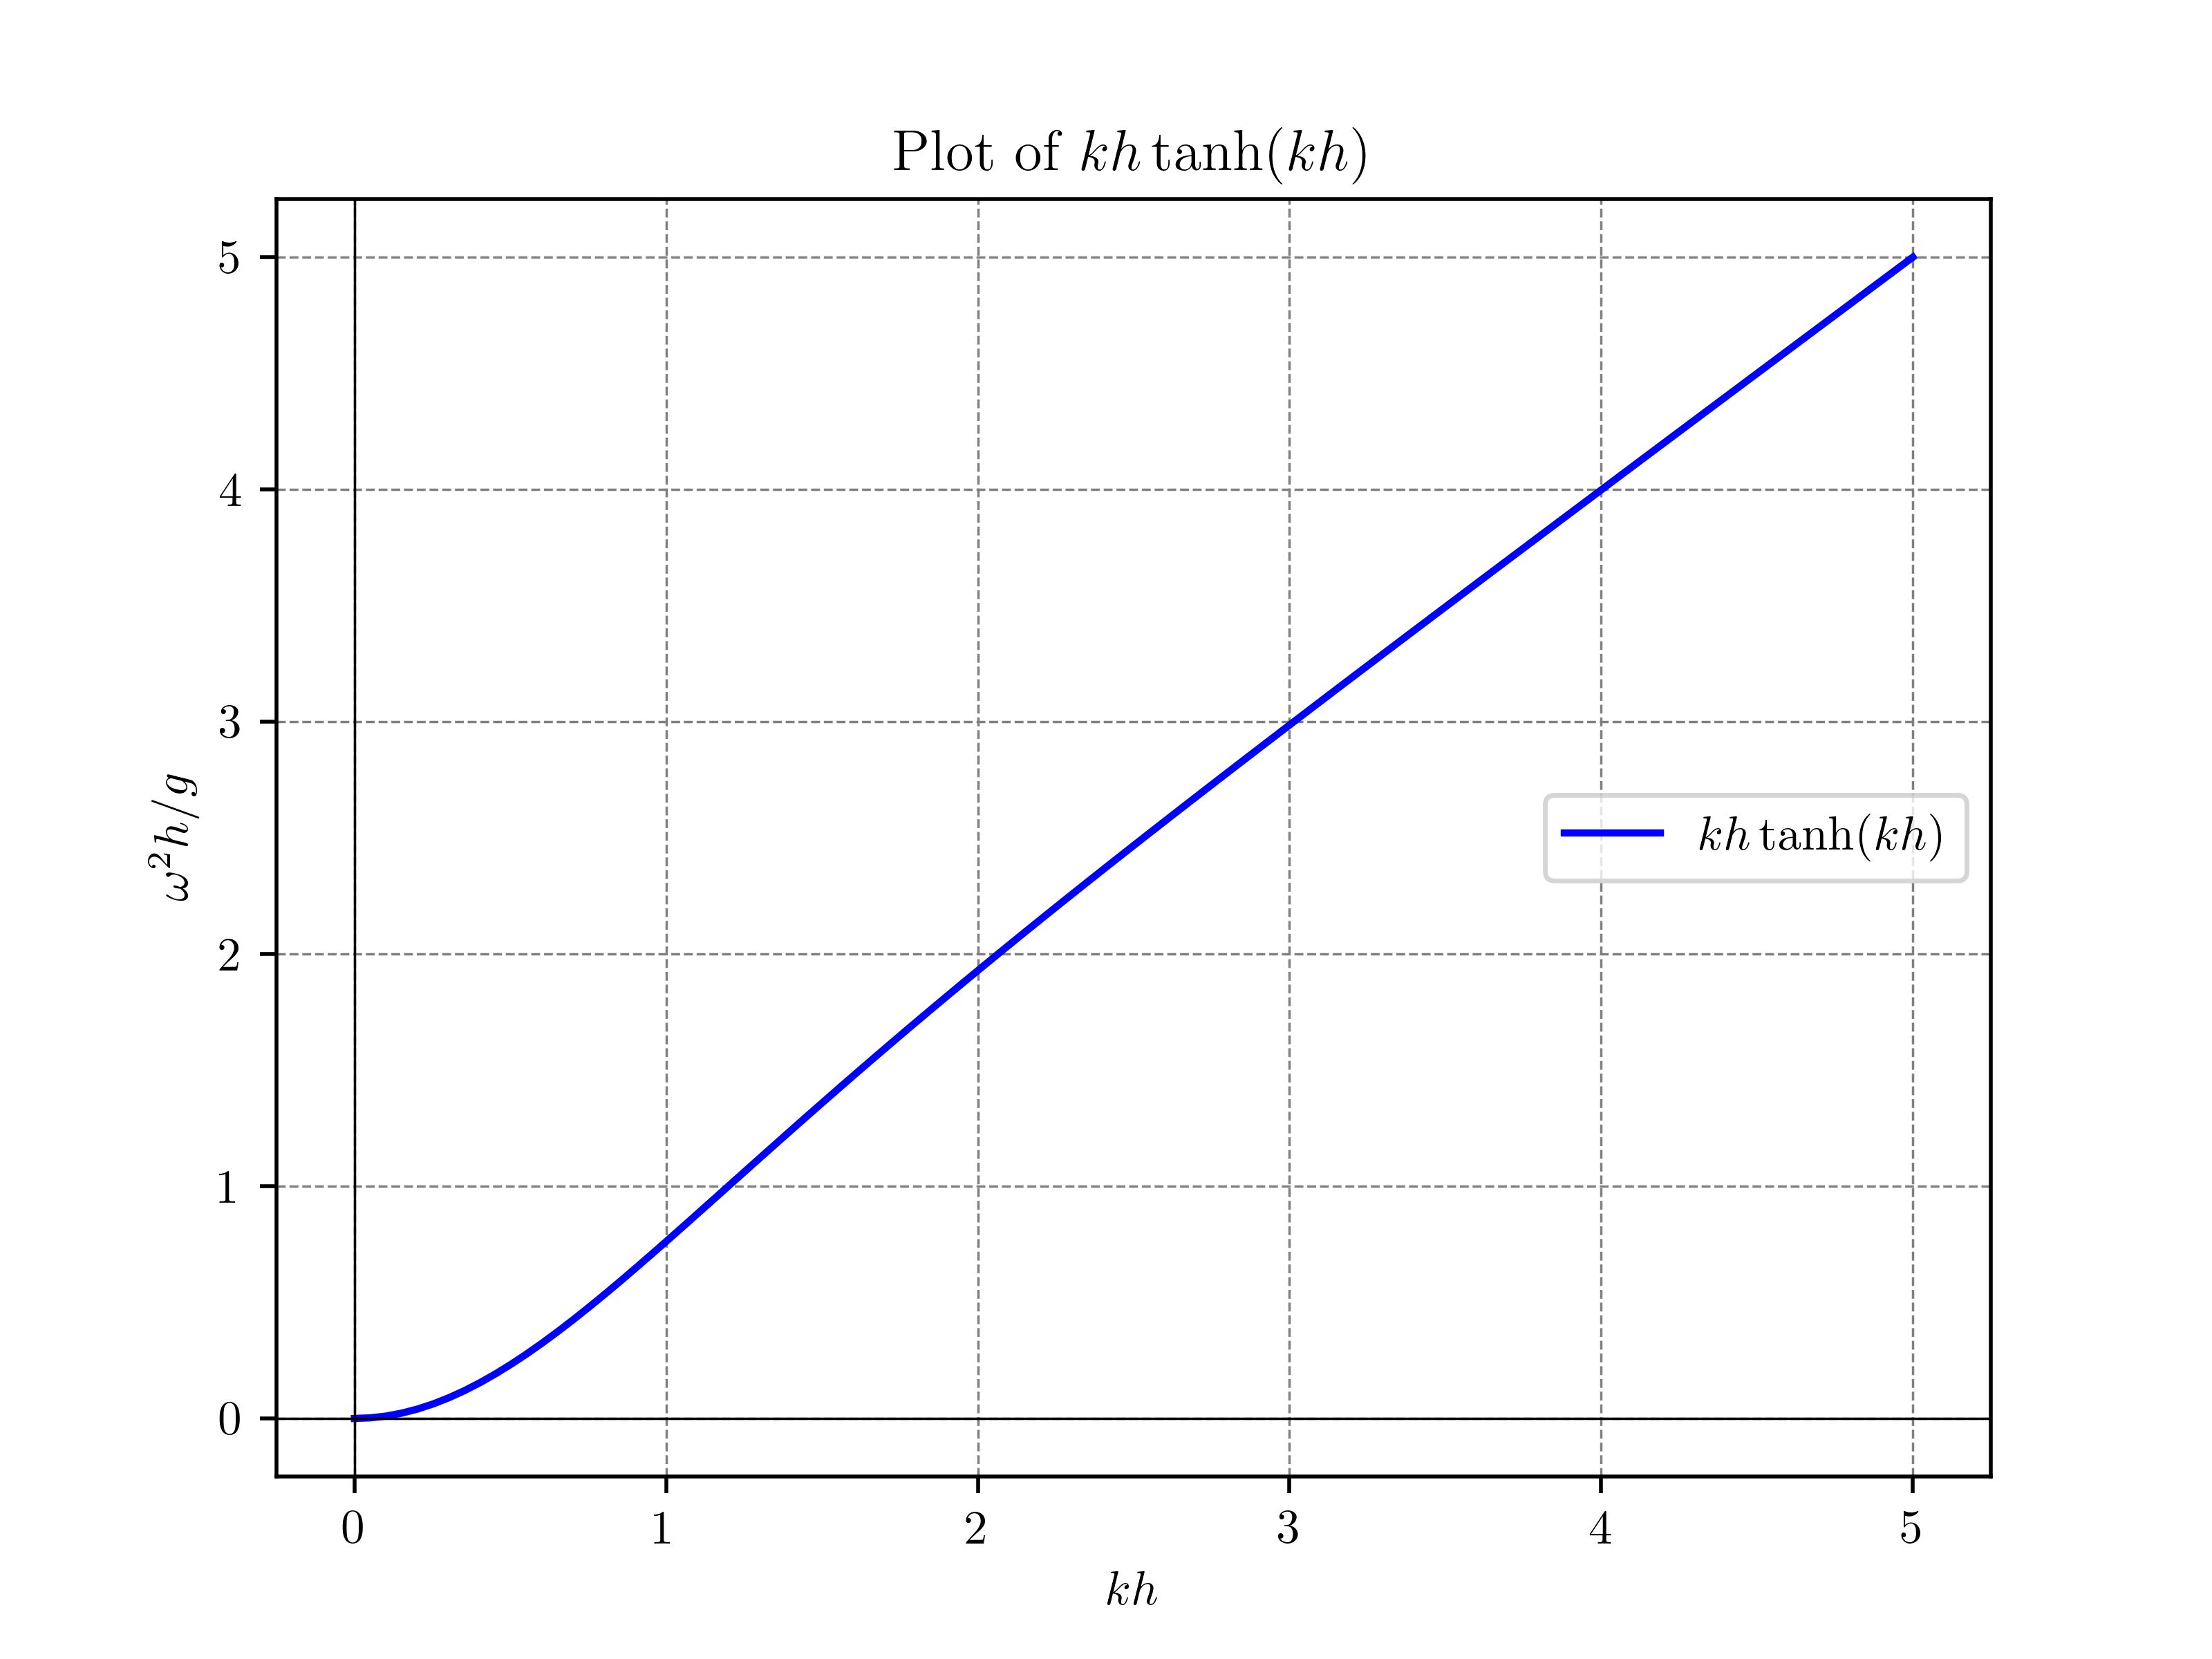
\includegraphics[width=0.7\linewidth]{plot12161}
		\caption{}
		\label{fig:plot12161}
	\end{figure}
	\begin{figure}[H]
		\centering
		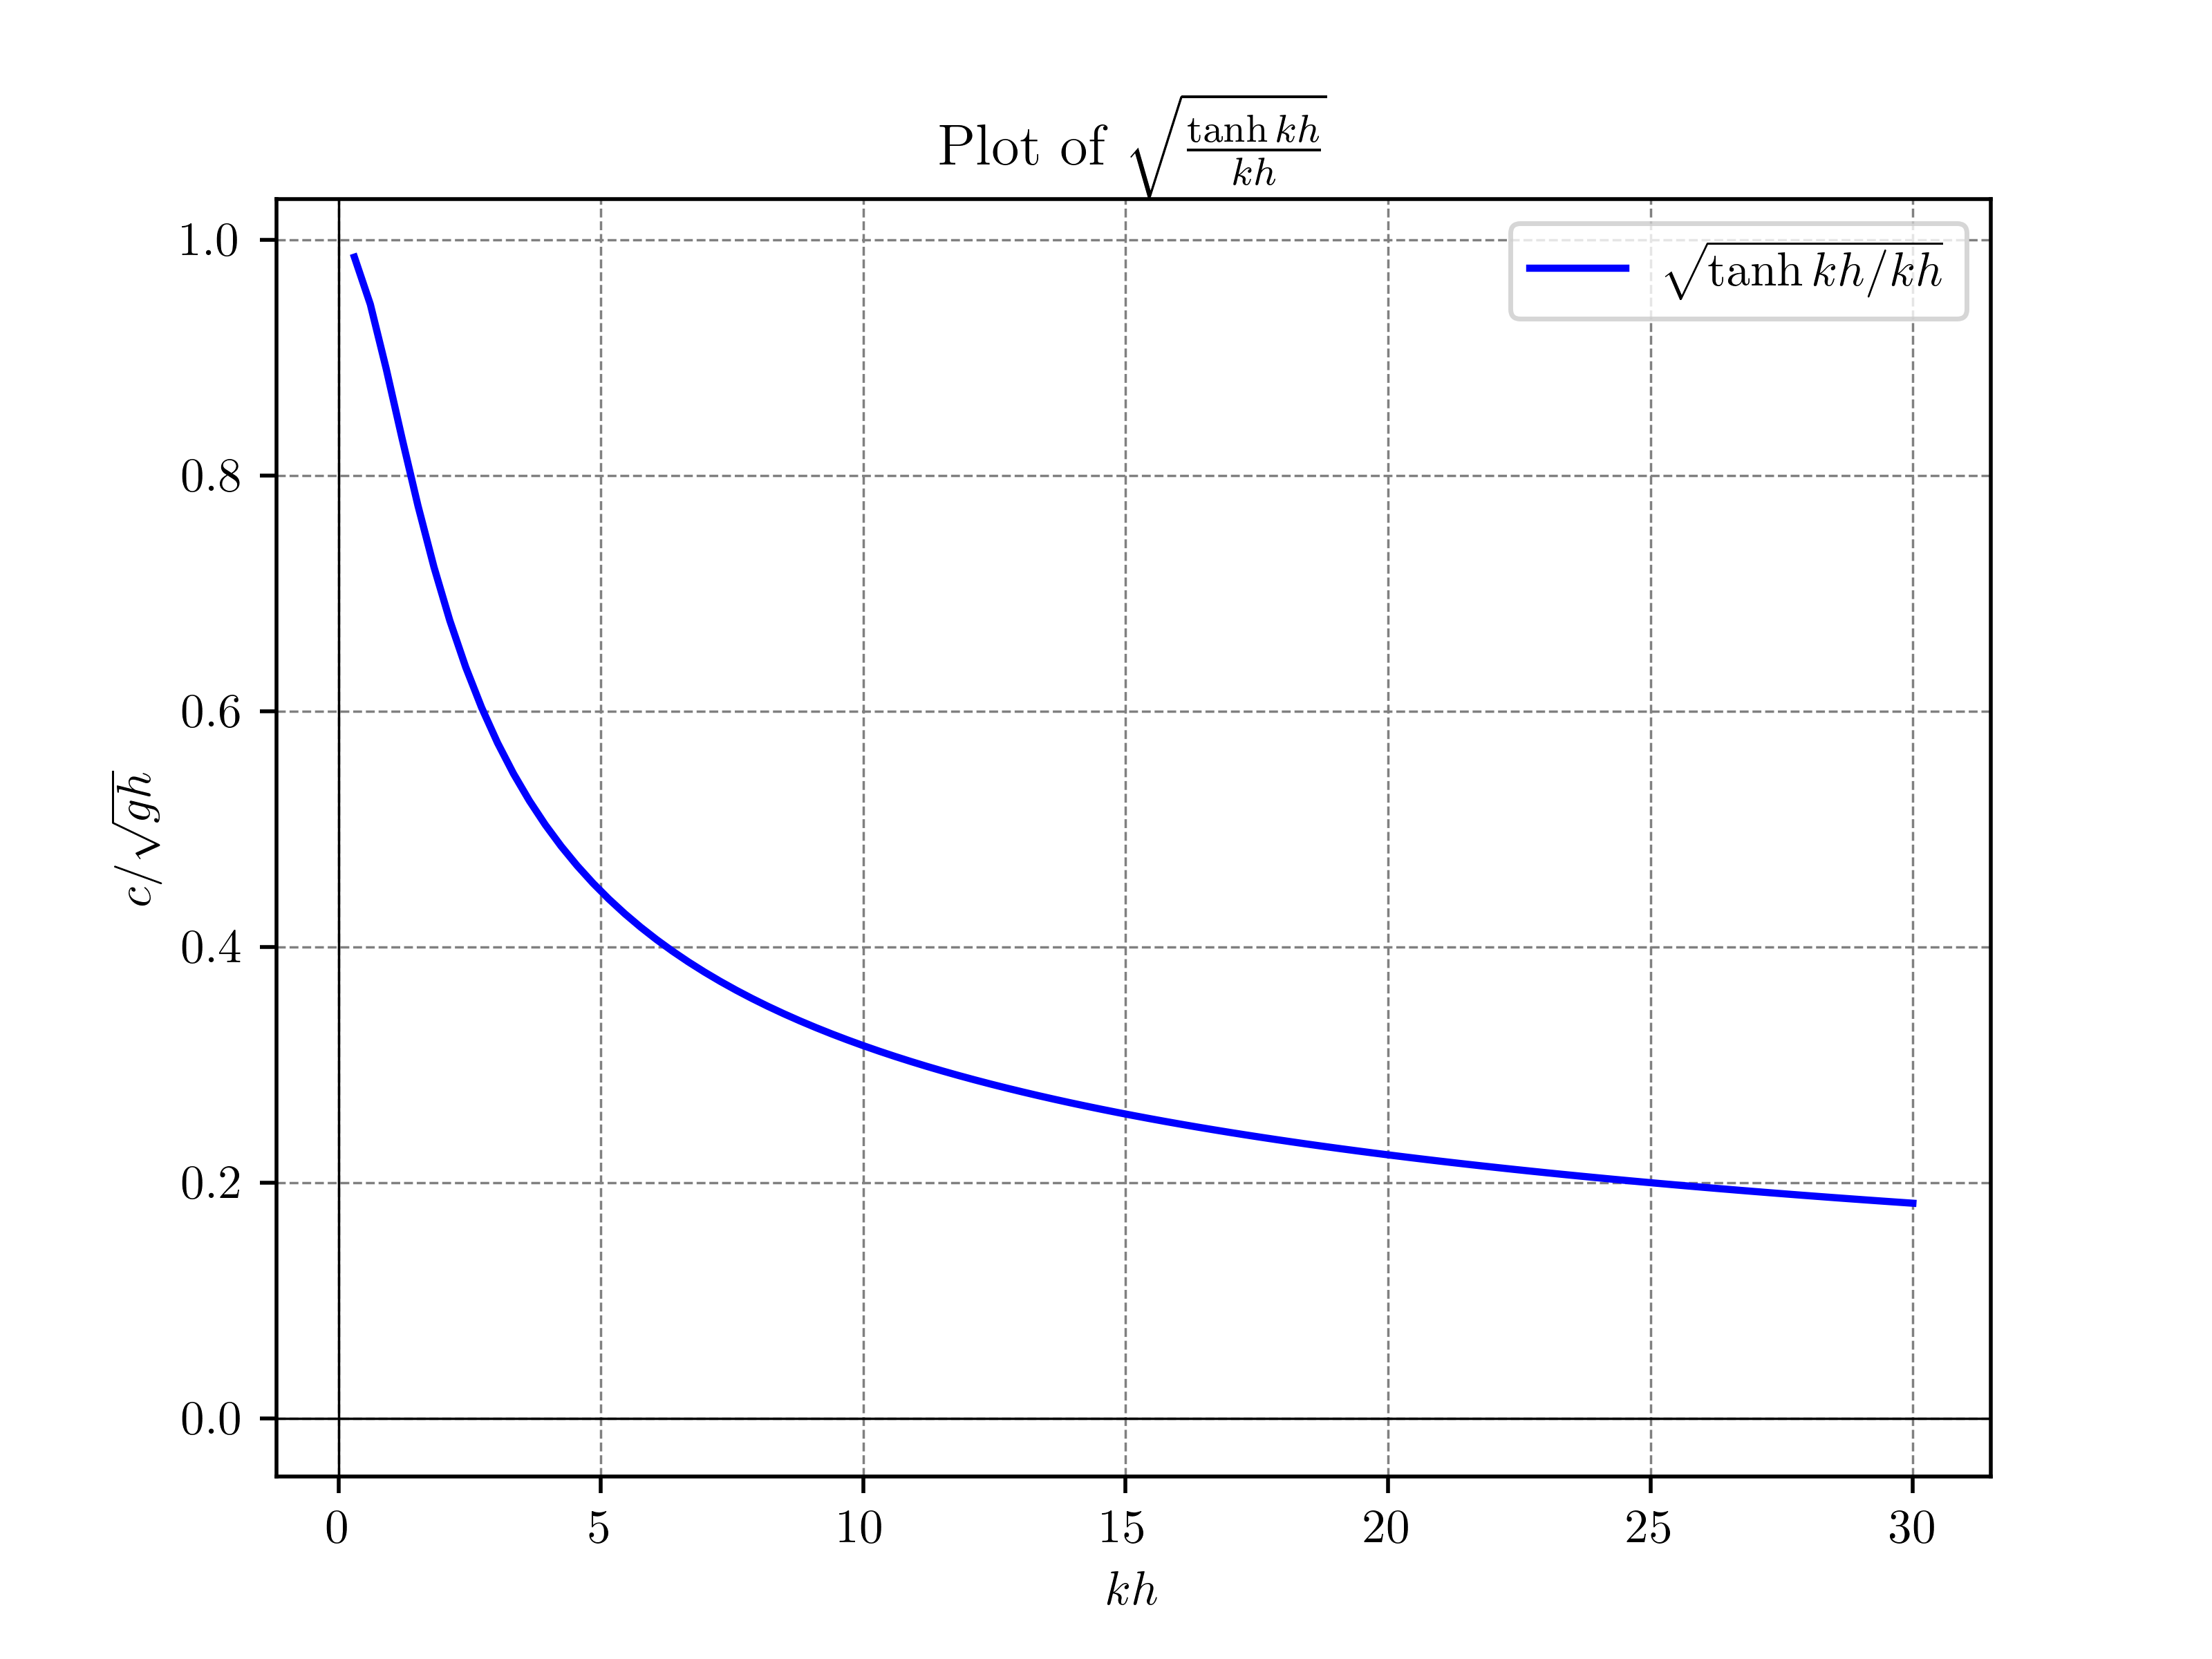
\includegraphics[width=0.7\linewidth]{plot12162}
		\caption{}
		\label{fig:plot12162}
	\end{figure}
		\section{Pressure from the Unsteady Bernoulli Equation}
	\subsection{Unsteady Bernoulli Equation}
	\begin{figure}[H]
		\centering
		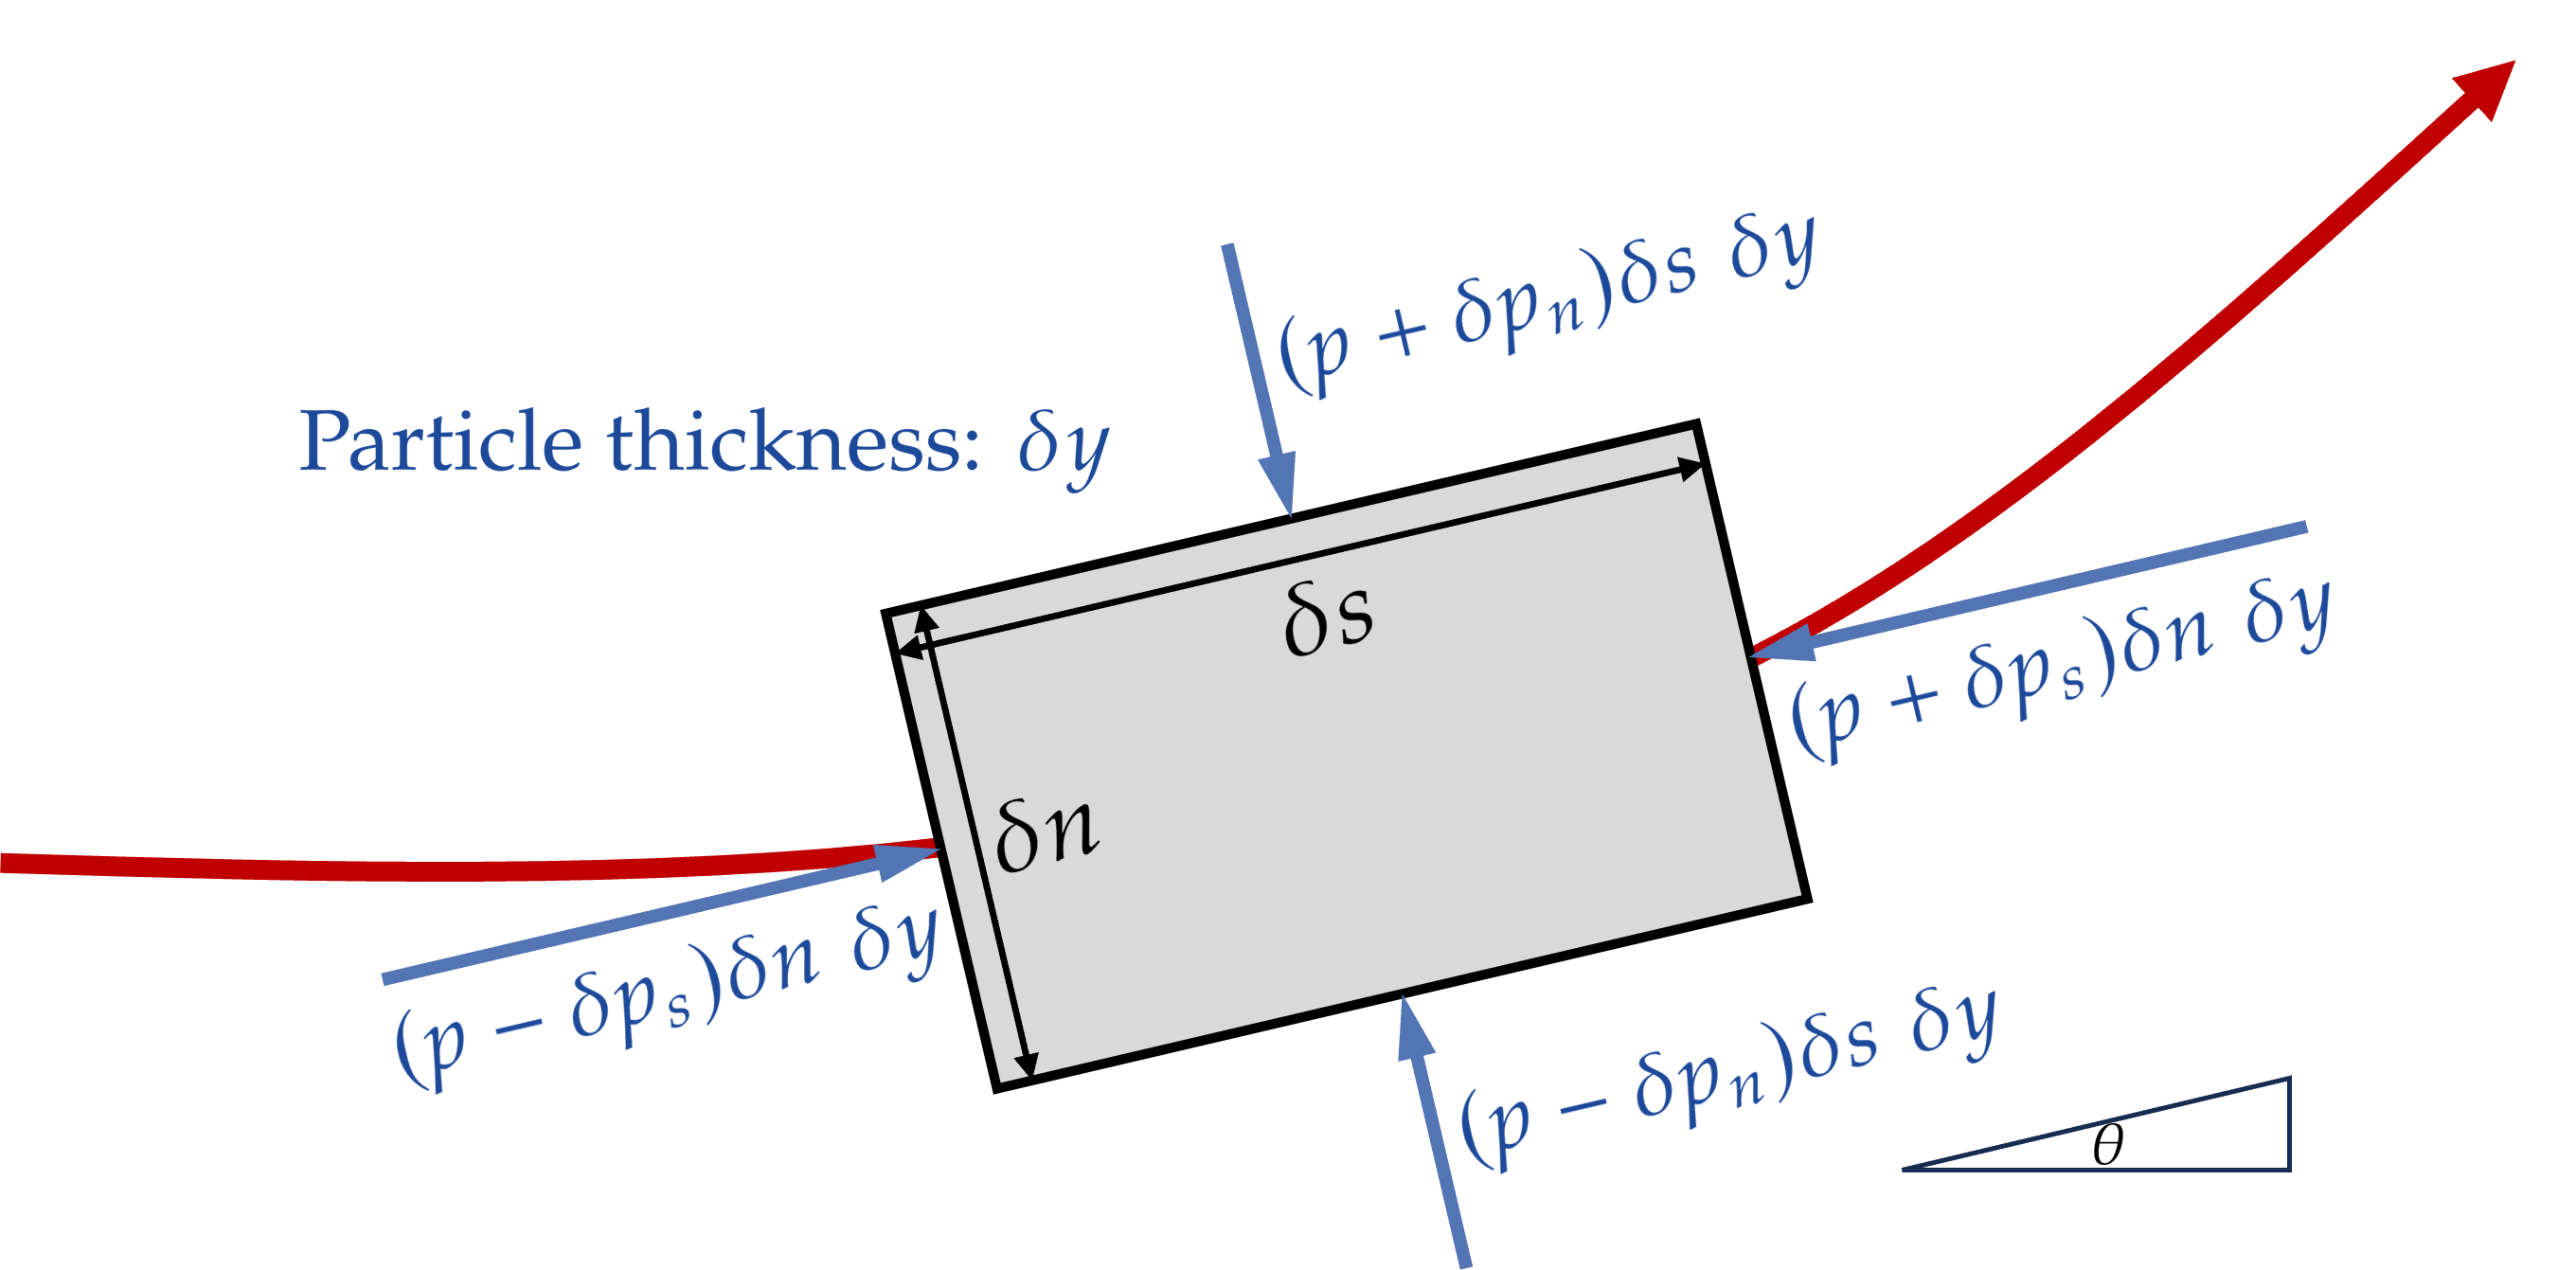
\includegraphics[width=0.7\linewidth]{unsteady}
		\caption{Small Fluid Particle Along a Streamline}
		\label{fig:unsteady}
	\end{figure}
	We first obtain the unsteady Bernoulli equation. We consider a small fluid 
	particle along a streamline of size $\delta s$ by $\delta n$ in the plain, 
	and denote forces exerted to the particle as above in Fig. 
	\ref{fig:unsteady}. $\delta p_s$ and $\delta p_n$ are respectively amounts 
	of the equal pressure differences of end faces parallel to the streamline 
	and 
	perpendicular to the streamline. We hereby write Newton's second law along 
	the streamline direction as follows:
	\begin{equation}
		\label{eq:new}
		\Sigma\, \delta F_s=\delta m\, a_s,
	\end{equation}
	where $a_s$ denotes acceleration along the streamline. We know that 
	velocity $V(s,t)$ is a function of 
	location in the streamline $s$ and time $t$. Accordingly, we write
	\begin{equation*}
		\Sigma\,\delta F_s=\delta m\left(\frac{\partial V}{\partial 
		t}+V\frac{\partial V}{\partial s}\right)=\rho \,\delta 
		V_{\mathrm{control}}\left(\frac{\partial V}{\partial 
		t}+V\frac{\partial V}{\partial s}\right). 
	\end{equation*}
	
	Meanwhile, $\Sigma\,\delta F_s=\delta W_s+\delta F_{ps}$ where $\delta W_s$ 
	is gravitational force along the streamline and $\delta F_{ps}$ is pressure 
	force along the streamline. We obtain $\delta W_s$ and $\delta F_{ps}$ from 
	force relations as follows:
	\begin{align*}
		\delta W_s&=-\delta W \sin \theta=-\gamma\, \delta 
		V_{\mathrm{control}}\sin \theta\\
		\delta F_{ps}&=(p-\delta p_s)\,\delta n\;\delta y-(p+\delta 
		p_s)\,\delta 
		n 
		\,
		\delta y=-2\,\delta p_s\,\delta p_n\,\delta y.
	\end{align*}
	
	Here, since we are considering a small particle, we can neglect higher 
	order terms from the pressure field, therefore $2\,\delta p_s\approx 
	(\partial p\,/\partial s)\;\delta s$. Inserting this result to $\delta 
	F_{ps}$ and Eq. (\ref{eq:new}) gives
	\begin{equation}
		\label{eq:force}
		\Sigma\,\delta F_s=\delta W_s+\delta 
		F_{ps}=\left(-\gamma\sin\theta-\frac{\partial p}{\partial 
		s}\right)\,\delta V_{\mathrm{control}}=\rho\left(\frac{\partial 
		V}{\partial t}+V\frac{\partial V}{\partial s}\right).
	\end{equation}
	
	Now integrating Eq. (\ref{eq:force}) gives us the unsteady Bernoulli 
	equation:
	\begin{equation}
		\label{eq:uns}
		p+\frac{1}{2}\rho V^2+\gamma z+\rho \frac{\partial \phi}{\partial t}=0.
	\end{equation}
	\subsection{Pressure from the Linearized Unsteady Bernoulli Equation}
	\begin{figure}[H]
		\centering
		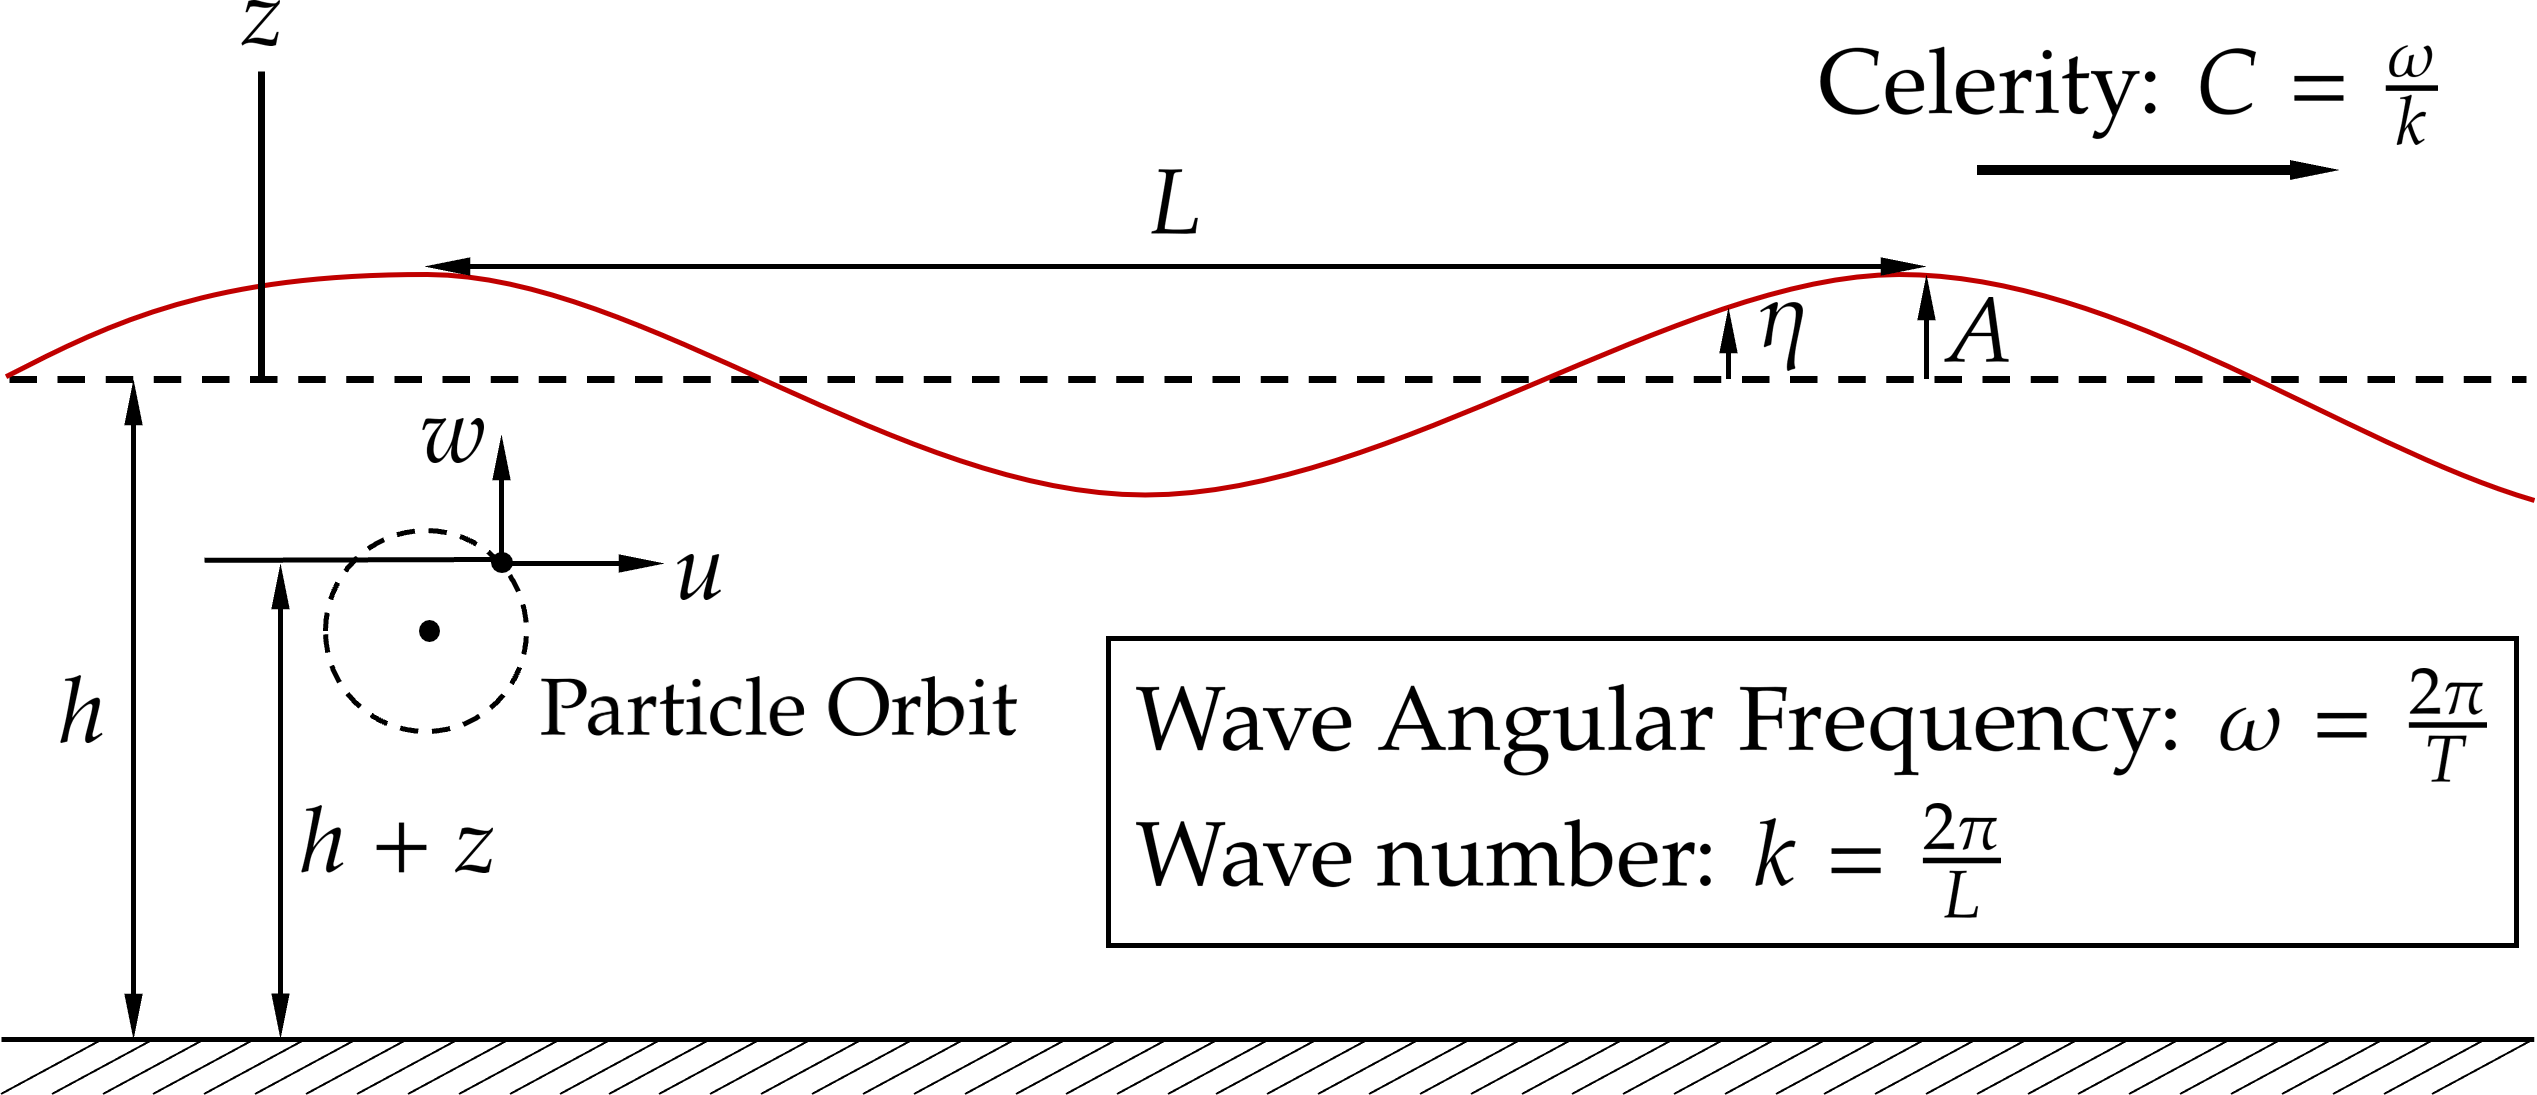
\includegraphics[width=0.7\linewidth]{surfacewave}
		\caption{Free Surface Waves}
		\label{fig:surfacewave}
	\end{figure}
We next apply the unsteady Bernoulli equation according to the notations given 
in Fig. \ref{fig:surfacewave} above:
	\begin{equation}
		\label{eq:ber}
		\frac{1}{2}(u^2+w^2)+\frac{P}{\rho}+gz+\frac{\partial \Phi}{\partial 
		t}=0,
	\end{equation}
	where $u$ and $w$ are each horizontal and vertical components of the water 
	particle velocity and $h$ is water depth.
	
	Here, we linearize and omit higher-order terms, then write $P$ as follows:
	\begin{equation}
		\label{eq:pressure}
		P=-\rho gz-\rho\frac{\partial\Phi}{\partial t}.
	\end{equation}
	
	Then we calculate $\partial\Phi/\partial t$:
	\begin{equation}
		\label{eq:der}
		\frac{\partial\Phi}{\partial t}=-gA\left[\frac{\cosh k(z+h)}{\cosh 
		kh}e^{i(kx-\omega t)}\right].
	\end{equation}
	
	Note that $\Phi$ here is a complex potential $\Phi=\phi+i\psi$, where
	\[\phi= \frac{gA}{\omega}\frac{\cosh k(h+z)}{\cosh kh}\sin(kx-\omega t),\]
	and $\psi$ is its complex conjugate potential. Now we insert Eq. 
	(\ref{eq:der}) to Eq. (\ref{eq:pressure}). We here insert the real part of 
	the derivative, therefore obtain:
	\begin{equation}
		\label{eq:pre}
		P=-\rho gz+\rho gA\left[\frac{\cosh k(z+h)}{\cosh 
		kh}\right]\cos(kx-\omega t).
	\end{equation}
	
	Here, we see that the first term on the right $-\rho gz$ gives us the 
	normal hydrostatic pressure variation relative to $z$ while the second term 
	indicates the dynamic pressure from particle acceleration induced by the 
	wave. 
	\section{Wave Train Propagation Over a Uniform Slope}
	\subsection{Plotting Wave Transformation}
	We first consider the group velocity of wave trains. Considering 
	consecutive waves with phases $\delta_1$ and $\delta_2$ respectively, we 
	may write the composite wave of the two waves as follows:
	\begin{align*}
	\eta_T=\eta_1+\eta_2&=A\cos{(kx-\omega t+\delta_1)}+A\cos (kx-\omega t 
	+\delta_2)\\
	&=2A\cos\left[\frac{1}{2}(k_1-k_2)x-
	\frac{1}{2}(\omega_1-\omega_2)t\right]\sin\left[\frac{1}{2}(k_1+k_2)x-
	\frac{1}{2}(\omega_1+\omega_2)t\right].
	\end{align*}
	
	Now we see that at $t=0$, nodes occur at
	\[x=\frac{\pi}{k_1-k_2},\frac{3\pi}{k_1-k_2},\cdots\]
	thus we define group velocity $C_G$ as follows:
	\begin{align}
		C_g=\frac{\mathrm{d}x_{\mathrm{node}}}{\mathrm{d}x}=\frac{\omega_1-\omega_2}{k_1-k_2}.\nonumber
	\end{align}
	As $\omega_1$ approaches $\omega_2$, 
	\begin{align}
		\label{eq:cg}
		C_g&=\frac{\mathrm{d}\omega}{\mathrm{d}k}=C-L\frac{\mathrm{d}C}{\mathrm{d}L}\\
		&=\frac{C}{2}\left[1+\frac{2kh}{\sinh 2kh}\right].
	\end{align}
	
	Now, we derive the energy of a wave. We first calculate the kinetic energy 
	for a unit width of wave crest and for one wave length, $E_k$. We calculate 
	as follows:
	\begin{align}
		\label{eq:ek}
		E_k=\int_0^L\int_{-d}^{0}\frac{1}{2}\rho\;\mathrm{d}x\,\mathrm{d}z(u^2+w^2)=\frac{\rho
		 gH^2L}{16}.
	\end{align}
	
	Now, if we subtract the potential energy of a mass of still water with 
	respect to the bottom from the potential energy of the wave form, this 
	gives the potential energy per unit wave crest width and for one 
	wavelength, $E_p$.
	\begin{align}
		\label{eq:ep}
		E_p=\int_0^L \rho 
		g(h+\eta)\left(\frac{h+\eta}{2}\right)\mathrm{d}x-\rho 
		gLd\left(\frac{d}{2}\right)=\frac{\rho
		 gH^2L}{16}.
	\end{align} 
	From Eqs. (\ref{eq:ek}) and (\ref{eq:ep}), we obtain total energy in a wave 
	per unit crest width $E$:
	\begin{align}
		\label{eq:e}
		E=E_k+E_p=\frac{\rho gH^2L}{8}.
	\end{align}
	\begin{figure}[H]
		\centering
		\includegraphics[width=0.7\linewidth]{final12171}
		\caption{Wave Propagation Towards the Shoreline}
		\label{fig:final12171}
	\end{figure}
	
	Assuming that over the distance $\Delta x$, regardless of its length, there 
	is no generation, reflection, and dissipation of wave energy, 
	\begin{align*}
		(EbC_G)_1=(EbC_G)_2,
	\end{align*}
	where $b$ is the width of the channel.
	
	From Eq. (\ref{eq:e}), we alternatively write as follows:
	\begin{align}
		\label{eq:econ}
		\frac{A^2 b}{4}\left[\frac{g}{k}\tanh 
		kh\right]^{1/2}\left[1+\frac{2kh}{\sinh 2kh}\right]=\textit{const.}
	\end{align}
	
	According to the fact that $C^2=\frac{g}{k}\tanh kh$, we may write
	\begin{equation}
		\frac{C}{C_0}=\frac{L}{L_0}=\frac{k_0}{k}=\tanh kh,
	\end{equation}
	where the subscript $_0$ indicates the value of the variable in deep water. 
	For instance, 	
	\begin{equation}
		C_0=\frac{gT}{2\pi}=\SI{15.61}{m/s} \qquad 
		L_0=\frac{gT^2}{2\pi}=\SI{156.13}{m}.
	\end{equation}
	
	Meanwhile, from Eq. (\ref{eq:econ}), we also obtain the relation
	\begin{equation}
		\frac{H}{H_0}=\left[\frac{b_0}{b}\right]^{1/2}\left[\frac{2\cosh^2 
		kh}{2kh+\sinh 2kh}\right]^{1/2}.
	\end{equation}
	
	Now combining the two relations, and assuming constant width of channel 
	$b=b_0$, we obtain an expression for the 
	transformation of wave steepness $kA=\pi H/L$:
	\begin{align}
		(kA)=(kA)_0\left[\frac{2\cosh^2 
		kh}{2kh+\sinh 2kh}\right]^{1/2}\coth kh.
	\end{align}
	
	Finally, we plot the desired physical variables in terms of $h/L_0$, in 
	order to provide a practical calculation method appliable for any $h$. From 
	the relation
	\begin{equation}
		kh=\frac{2\pi 
		h}{L}=\frac{h}{L_0}2\pi\frac{L_0}{L}=\left(\frac{h}{L_0}\right)2\pi\frac{1}{\tanh
		 kh},
	\end{equation}
	we easily substitue $kh$ in terms of $h/L_0$. Plots obtained are as follows.
	\begin{figure}[H]
		\centering
		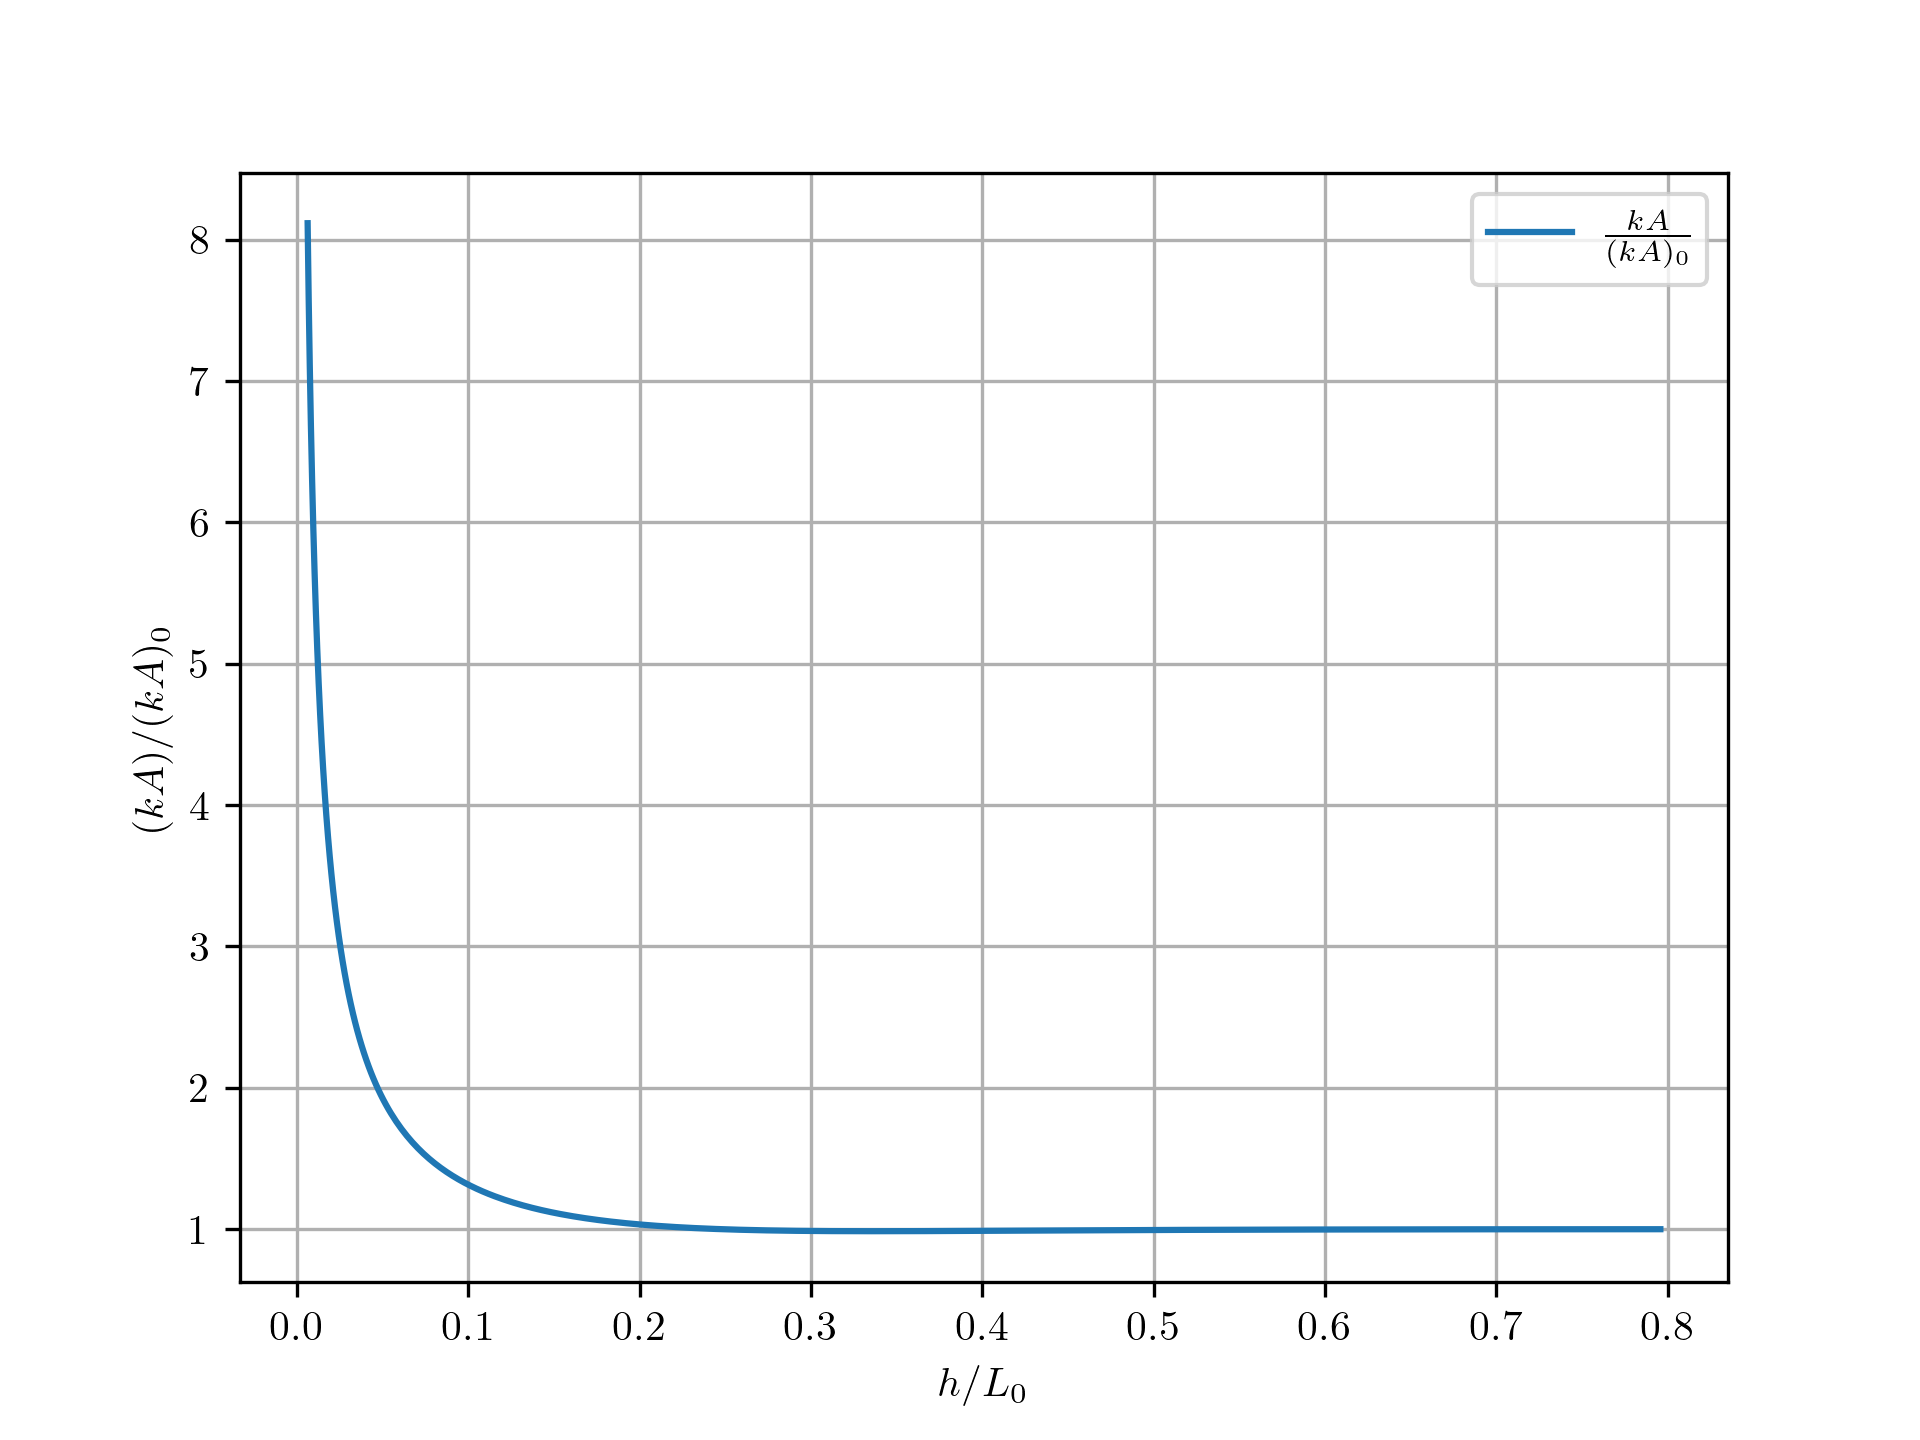
\includegraphics[width=0.7\linewidth]{plot12181}
		\caption{Wave Steepness Transformation}
		\label{fig:plot12181}
	\end{figure}
	\begin{figure}[H]
		\centering
		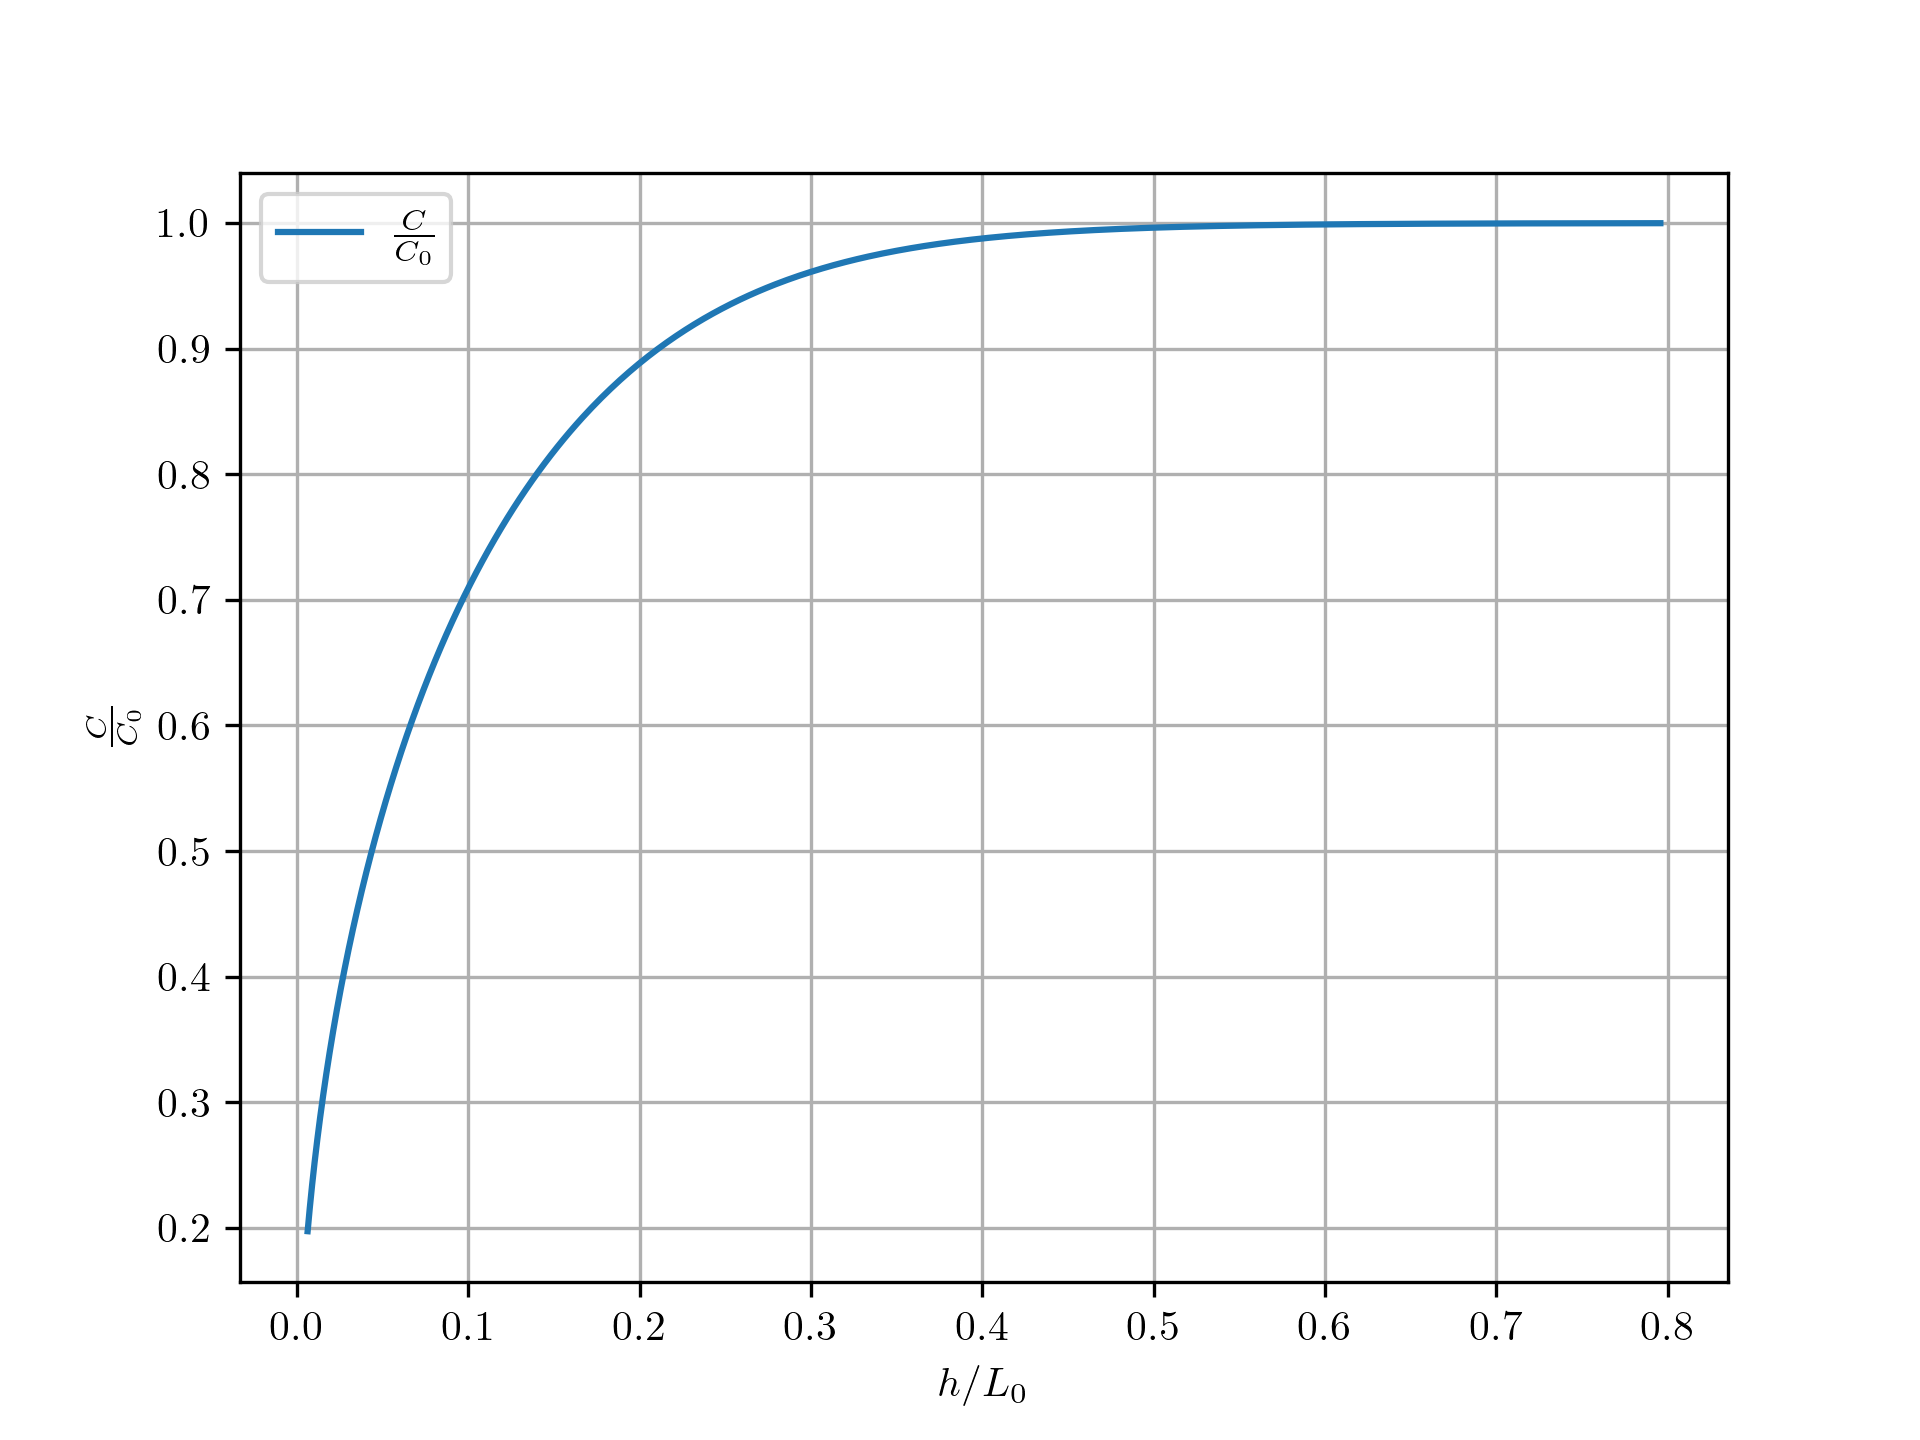
\includegraphics[width=0.7\linewidth]{plot12182}
		\caption{Celerity Transformation}
		\label{fig:plot12182}
	\end{figure}
	\begin{figure}[H]
		\centering
		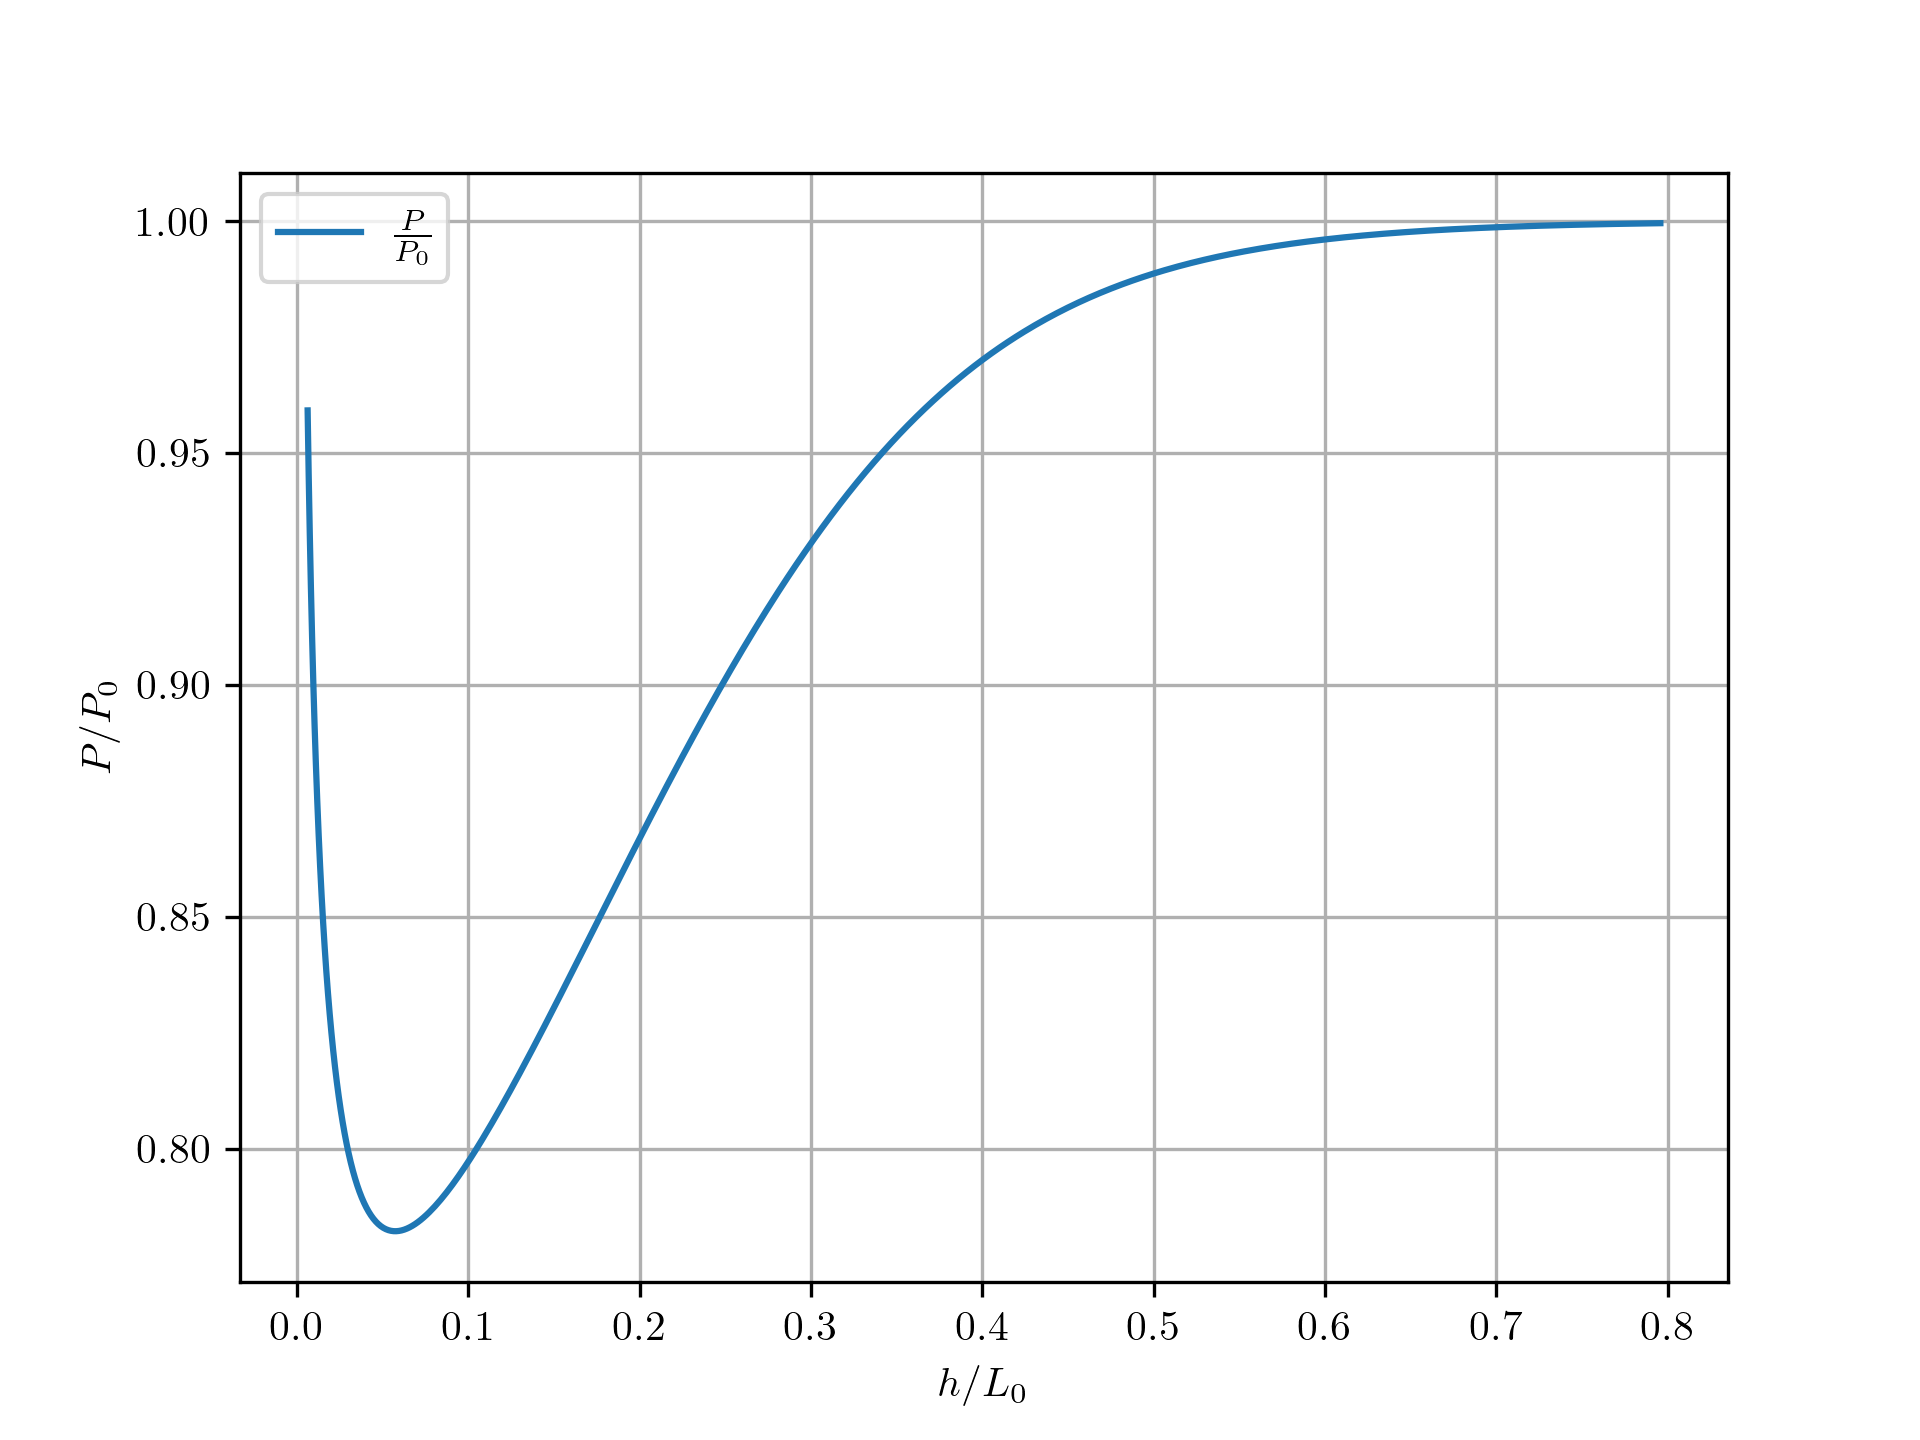
\includegraphics[width=0.7\linewidth]{plot12183}
		\caption{Dynamic Pressure Tranformation}
		\label{fig:plot12183}
	\end{figure}
	\begin{figure}[H]
		\centering
		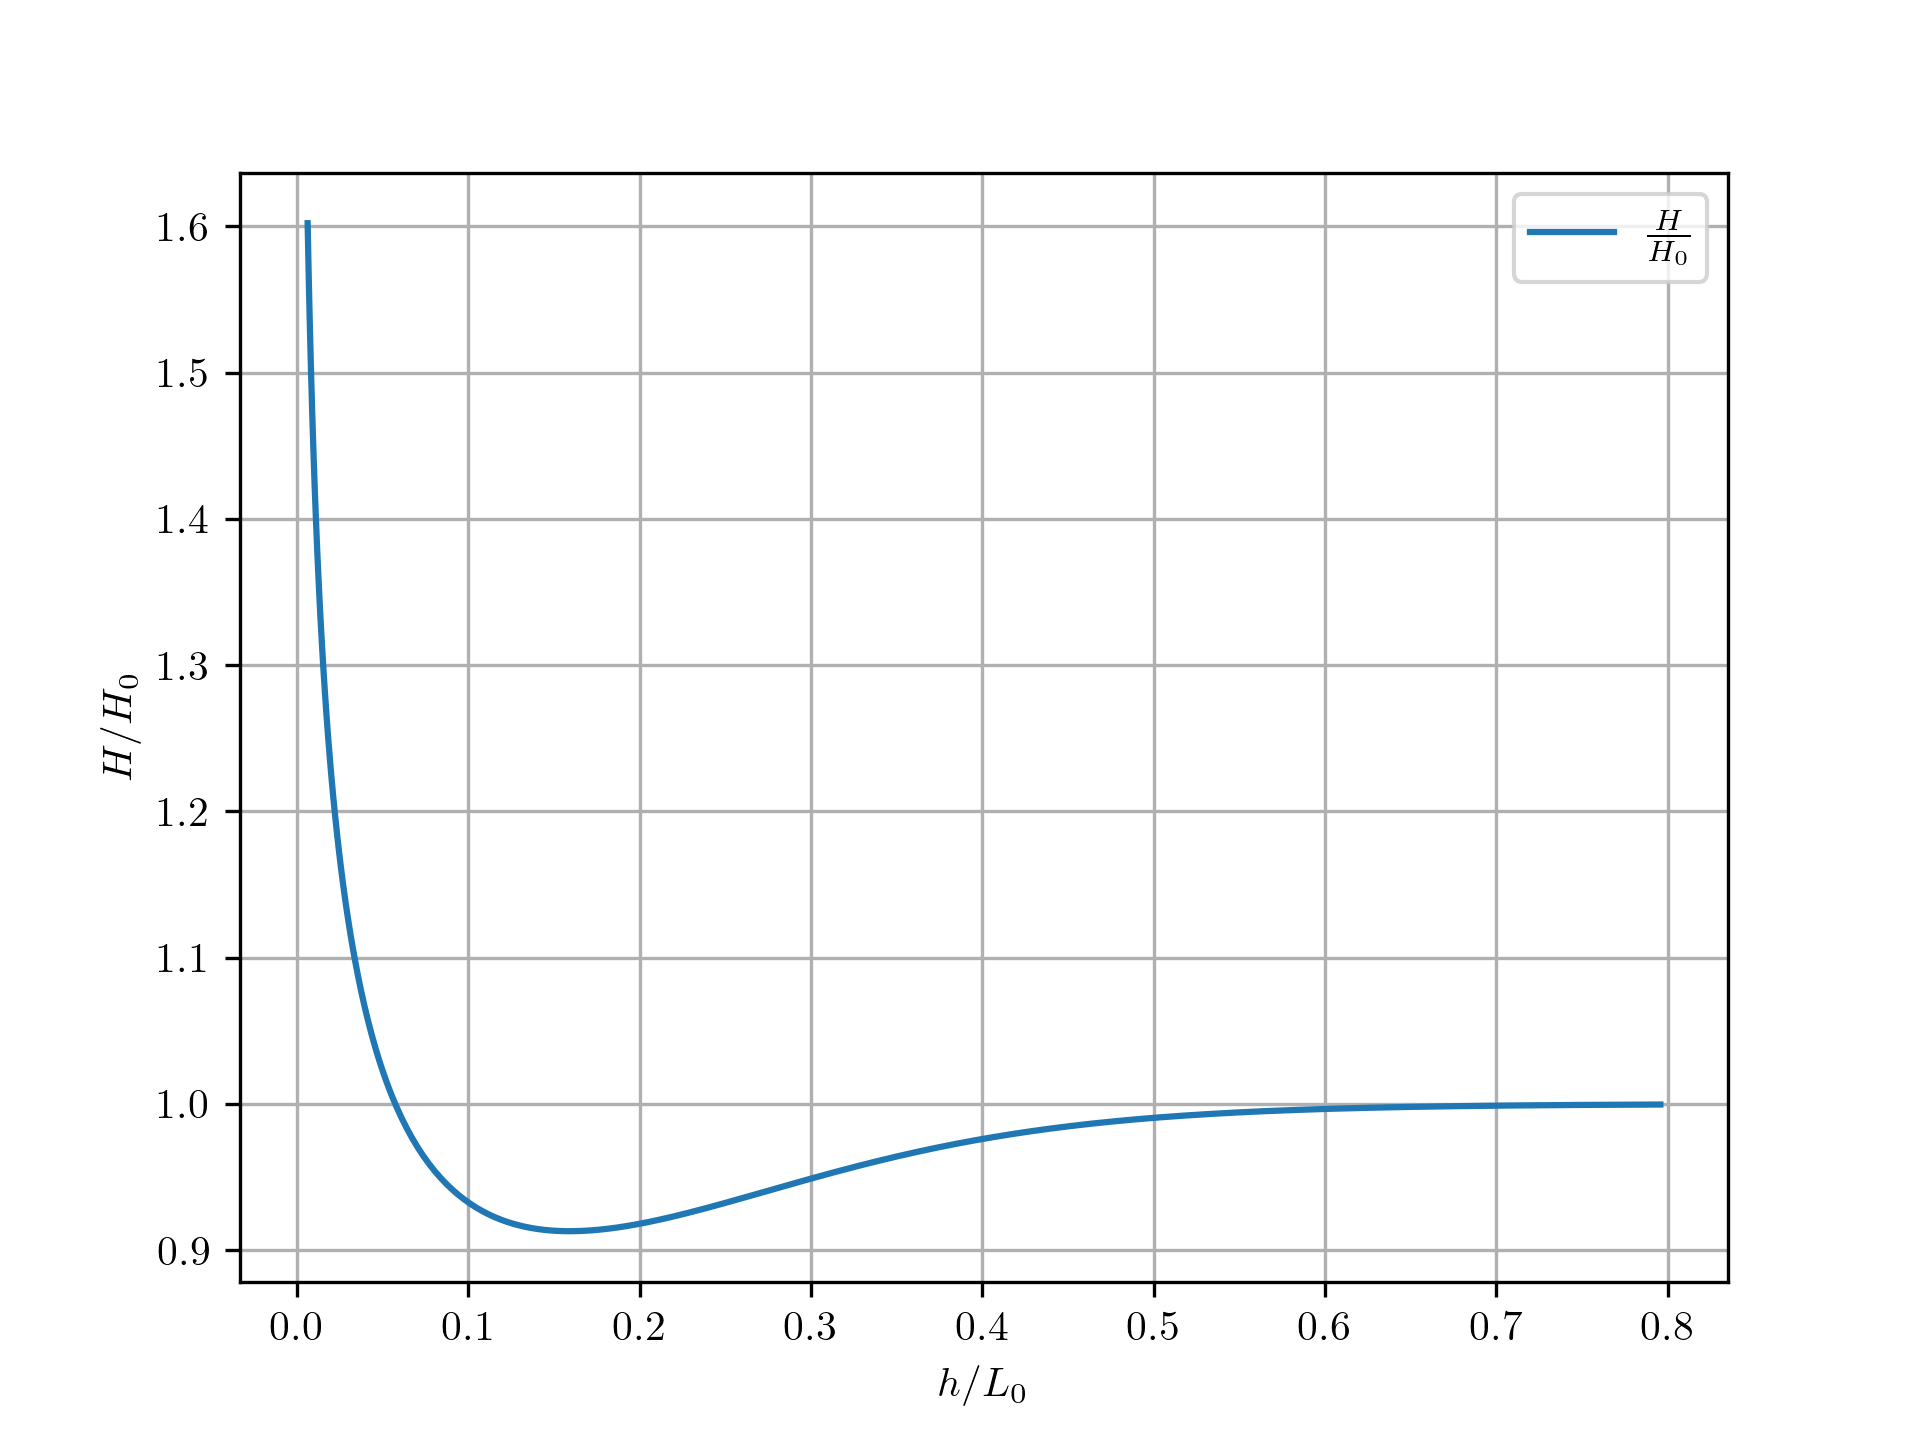
\includegraphics[width=0.7\linewidth]{plot12184}
		\caption{Amplitude Transformation}
		\label{fig:plot12184}
	\end{figure}
	\subsection{Observations of the Plots}
	\begin{enumerate}
	\item We realize that wave steepness $kA$ gets significantly higher when 
	approaching the shore, which in reality would break before reaching a 
	certain point, as wave becomes unstable.
	\item $C/C_0$ is proportional to $\tanh kh$, as shown in the plot.
	\item We examine that the ratio $P/P_0$ converges in deep water, while 
	reaching a certain minimum as reaching the shore, then rises again.
	\item Amplitude transformation is as Fig. \ref{fig:plot12184}, which also 
	reaches minimum in $h/L_0=0.157$, $H/H_0=0.91$. As mentioned, wave breaks 
	before amplitude rises infinitely.
	\end{enumerate}
	
		For slope of this instance, the small amplitude theory is satisfactory 
		for the prediction of phase velocity, until the point of wave breaking.
	
	In shallow water, the wave speed depends on the water depth, and waves with 
	different frequencies travel at different speeds, bound to the dispersion 
	relation. As waves propagate into shallower water, the longer wavelengths 
	travel faster than the shorter wavelengths, leading to a distortion of the 
	wave shape. Non-linear effects, such as wave steepening and wave breaking, 
	become more pronounced.
	
	For accurately modeling wave behavior in shallow water, more complex models 
	that consider non-linear effects, dispersion, and interactions with the 
	seabed are often employed. 
	
	While the linear assumption becomes less accurate as waves enter shallow 
	water, for a more precise analysis of wave behavior in shallow water, it is 
	necessary to consider non-linear effects.
\end{document}
